% LaTeX Template for short student reports.
% Citations should be in bibtex format and go in references.bib
\documentclass[a4paper, 11pt]{article}
\usepackage[top=3cm, bottom=3cm, left = 2cm, right = 2cm]{geometry} 
\geometry{a4paper} 
\usepackage[utf8]{inputenc}
\usepackage{textcomp}
\usepackage{graphicx} 
\usepackage{amsmath,amssymb}  
\usepackage{bm}  
\usepackage[pdftex,bookmarks,colorlinks,breaklinks]{hyperref} 
\usepackage{listings} 
%\hypersetup{linkcolor=black,citecolor=black,filecolor=black,urlcolor=black} % black links, for printed output
\usepackage{memhfixc} 
\usepackage{pdfsync}  
\usepackage{fancyhdr}
\usepackage[dvipsnames]{xcolor}
\pagestyle{fancy}

\usepackage{hyperref}
\hypersetup{
    colorlinks = false,
    linkbordercolor = {white},
}

\title{Project for Algorithms for Massive Datasets}
\author{Lukas Hirsch}
\date{}

\begin{document}
\maketitle
\vspace{13cm}
\noindent\makebox[\textwidth][c]{%
    \begin{minipage}{0.8\textwidth}
        I declare that this material, which I now submit for assessment, is entirely my own work and has not been taken from the work of others, save and to the extent that such work has been cited and acknowledged within the text of my work. I understand that plagiarism, collusion, and copying are grave and serious offences in the university and accept the penalties that would be imposed should I engage in plagiarism, collusion or copying. This assignment, or any part of it, has not been previously submitted by me or any other person for assessment on this or any other course of study.
    \end{minipage}}

\pagebreak
\tableofcontents
\pagebreak

\section{Introduction}
    In this report for the project of the course \textit{"Algorithms for Massive Datasets"}, the dataset of \textit{Letterboxd} \cite{Letterboxd}, a social network for sharing movie tastes, is used to train a deep learning model. The goal is to predict the genre of a movie based on its poster image. To achieve this, the image processing capabilities of the \textit{LeNet Convolutional Neural Network (CNN)} architecture are utilized. The model is trained with the movie posters provided in the \textit{Letterboxd} dataset, adapting the model to accurately predict genre from visual content. It is assumed that there is sufficient information in the poster for the classification to work well. This is a non-trivial problem as the visual content generally has to be translated into a suitable representation. Furthermore, the genre is an ambiguous label as there are films that belong to several genres at the same time. This project demonstrates the application of advanced image processing techniques to solve a big data problem in the field of movie classification. Everything in this project refers to the data set as of the 17.05.2024.

\section{Data Preparation}
    To use the data for further training, the posters and corresponding \textit{csv-file} for the genres were imported from the dataset. To prepare this data for effective use, it needs to be transformed into a suitable representation. In general, the csv files were read using the \textit{Python} library \textit{pandas}. For the images, \textit{read\_image} from the \textit{torchvision} library was used with a preprocessing pipeline. The link between them is a \textit{id} for each movie. For this, the genre table was grouped by the \textit{id} to make the id unique and to organize the genres as a list for each movie. All records missing either the image or the genre information were dropped.\\\\
    The specific preprocessing of the images included a resizing of the images to the general shape of (3, 345, 230). All images with only one channel were converted to \textit{rgb}, simply by repeating the value 3 times. Since there are not many of these images in the dataset, this dirty approach is appropriate. In addition, all posters were normalized to a mean of 0 and a standard deviation of 1 to improve the stability and generalization capabilities of the model later during training.\\\\
    On the other hand, handling the genre information requires a different approach. Given the limited number of unique genres in the dataset, one-hot encoding is an appropriate method to represent this categorical data. It is therefore transformed into binary vectors, where each genre is represented by a unique position in the vector. If a movie belongs to a certain genre, the corresponding position in the vector is set to 1, while all other positions with genres the movie doesn't belong to are set to 0. This binary representation ensures that the genre information is captured accurately and can be easily interpreted by the model.\\\\
    The number of data has been greatly reduced by sampling a fixed number of data points to limit processing time and memory usage. A sufficiently large number was chosen to reduce noise. 
    Data visualizations have shown that the distribution of the labels is very uneven, with dramas being heavily overrepresented (see fig. \ref{fig:unbalanced_data}), which can lead to problems during training. Regardless of the input, the model will predict the overrepresented class more often, first small training tests confirmed this. Consequently, while the model may achieve high overall accuracy due to the dominance of the majority class, it is likely to perform poorly on the minority classes.
    To compensate for this, a separate sampling procedure was implemented in advance to guarantee a minimum number of labels in the training dataset. This should prevent the minor classes from being neglected during training. The drama class is still the most dominant label in the data set but is significantly smaller in absolute terms (see fig. \ref{fig:balanced_data}). To ensure a meaningful evaluation of the performance at the end, this balanced data was only used during training. The normal randomly rebalanced sampled data was used for testing.\\
    \begin{figure}[h!]
        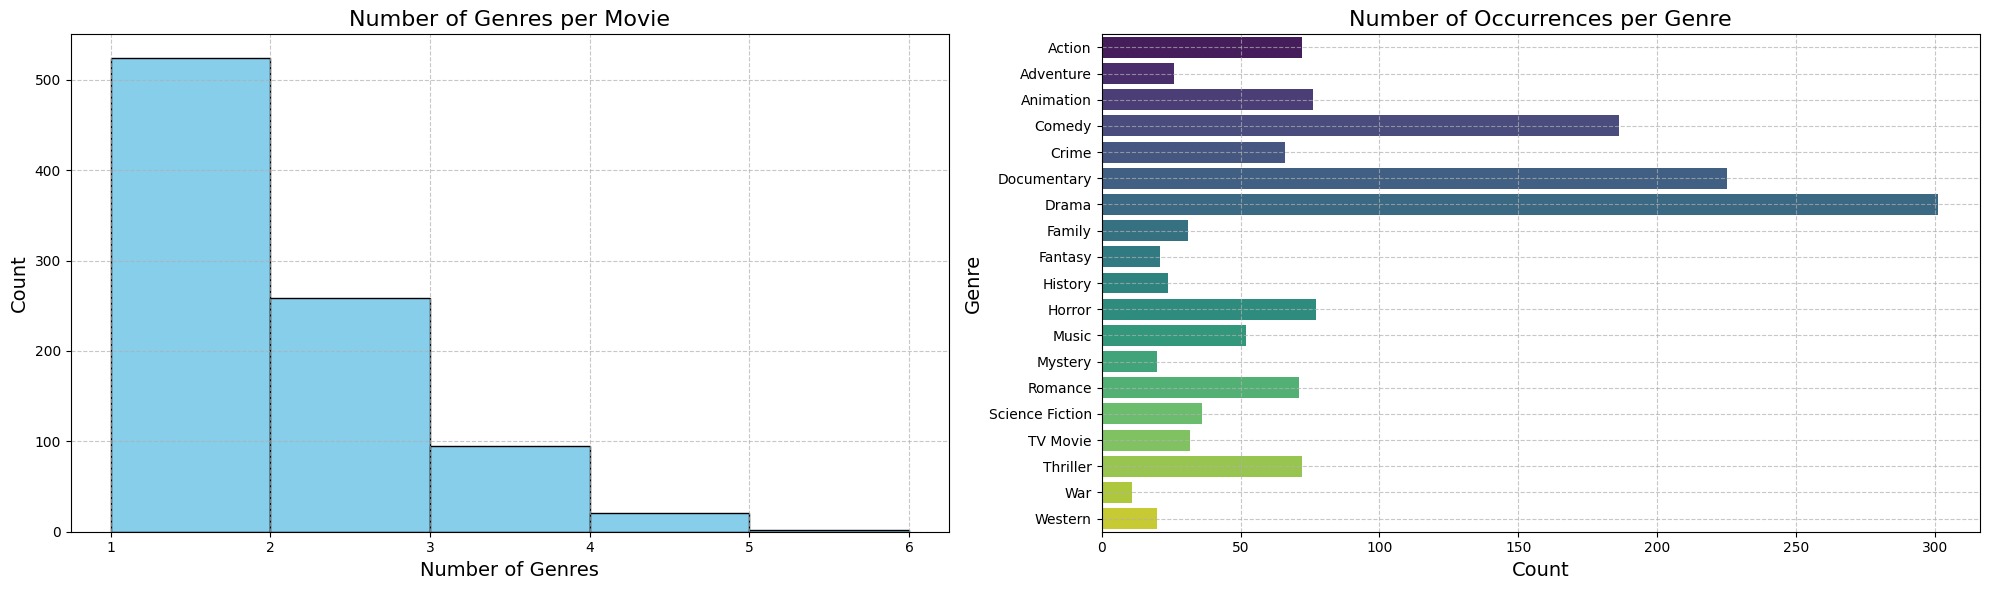
\includegraphics[width=\linewidth]{imgs/unbalanced_test_data.png}
        \caption{Example of initial unbalanced label distribution}
        \label{fig:unbalanced_data}
    \end{figure}
    \begin{figure}[h!]
        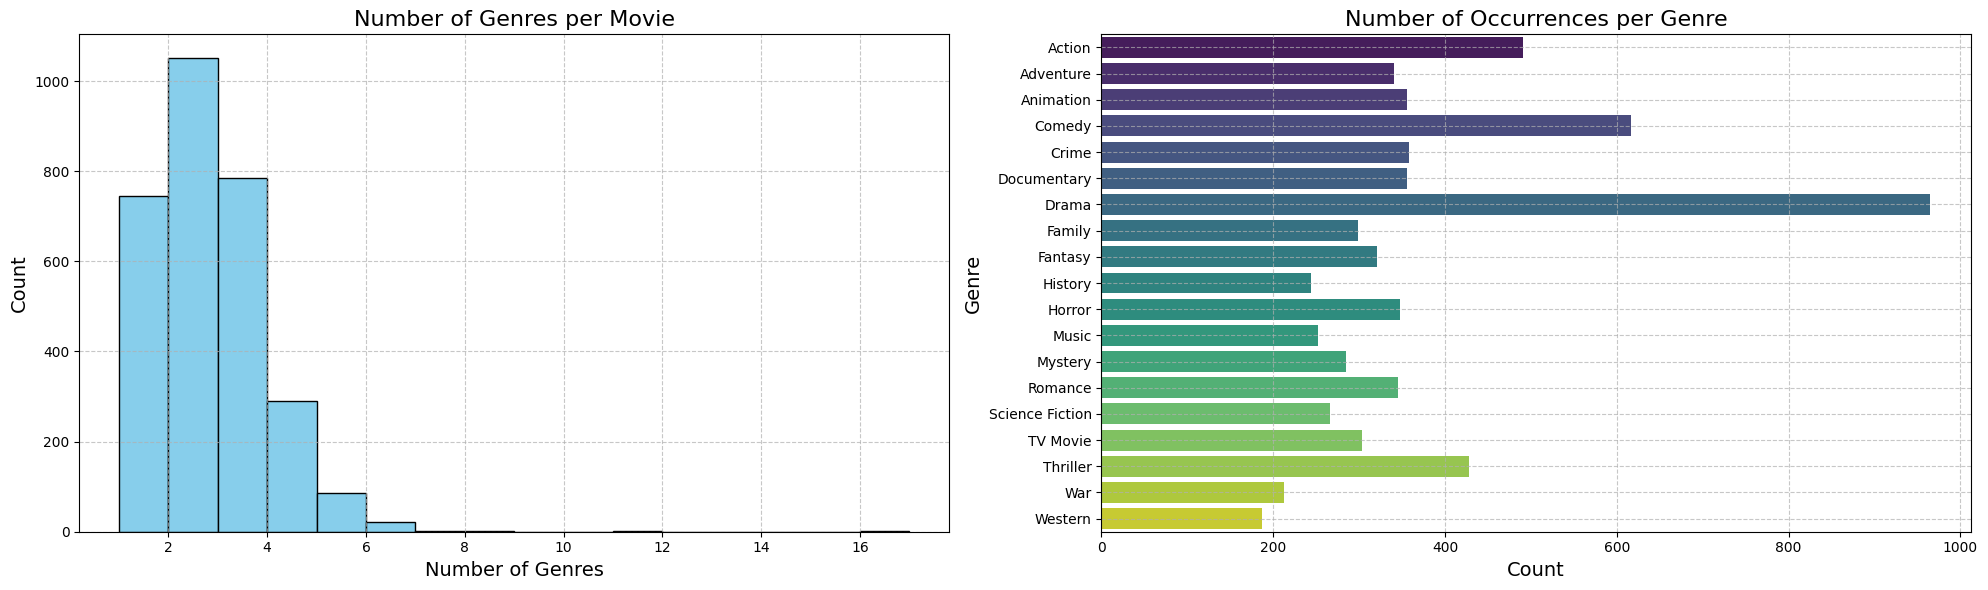
\includegraphics[width=\linewidth]{imgs/balanced_train_data.png}
        \caption{Example of balanced label distribution after pre-processing}
        \label{fig:balanced_data}
    \end{figure}
    \begin{figure}[h!]
        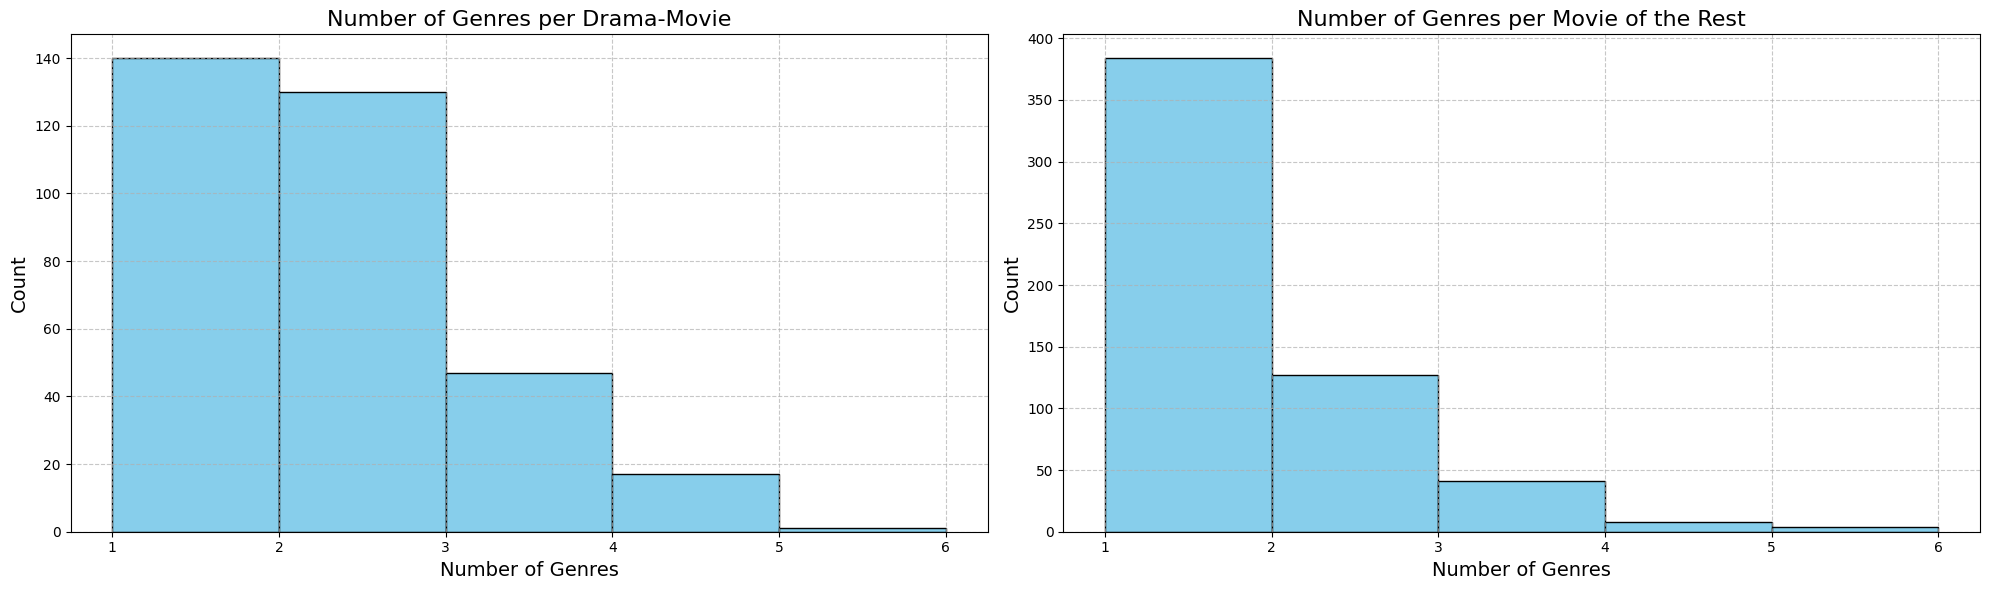
\includegraphics[width=\linewidth]{imgs/drama_distribution.png}
        \caption{Distribution of the number of genres for drama movies}
        \label{fig:drama_distribution}
    \end{figure}\\
    In the balanced dataset, a notable observation is the shift in the number of genres per film. This shift occurs because dramas are often more likely to span multiple genres than films in other categories (see fig. \ref{fig:drama_distribution}).
    When sampling to ensure a minimum representation of each genre, films with multiple genres are more likely to be included in the dataset.
    As a result, the process of balancing the dataset inadvertently favors multi-genre films. For example, a drama film might also be classified as a romance film, thus covering multiple genre categories. This multi-genre characteristic of dramas means that they have a higher probability of being selected during the balancing process to ensure that the minimum number requirements for each genre are met.
    This tendency can lead to a skewed representation where multi-genre films, especially those that include drama, dominate the dataset. Consequently, while balancing the dataset helps to mitigate the overrepresentation of any single genre, it introduces a bias toward multi-genre films. This bias needs to be carefully managed to ensure that the machine learning model trained on this dataset generalizes well and performs accurately across all genre categories, not just the multi-genre or drama-influenced ones.

\section{Methodology}
    The pre-processed data, consisting of the balanced training data set, balanced validation data set, and the unbalanced test data set, was then converted into a \textit{PyTorch} \textit{Dataset} for further processing. The batch size for later training is also set here, and is deliberately kept small to reduce the risk of overfitting. Possibly due to the noise they introduce into the learning process, small batches can provide a regularizing effect. This noise can help the model generalize better by preventing it from overfitting to the training data.\\\\
    \textit{LeNet} was chosen as the model architecture because it is one of the earliest and most influential \textit{CNN} architectures, developed by Yann LeCun and his colleagues in the late 1980s and early 1990s \cite{726791}. It was chosen for its simplicity and effectiveness. The used, slightly modified, version five has the following architecture:
    \begin{enumerate}
        \item \textbf{Input Layer}: Takes a 345x230 pixel \textit{rgb} image with 3 channels.
        \item \textbf{Convolutional Layer}: Applies six 5x5 filters, resulting in six 341x226 feature maps.
        \item \textbf{Subsampling Layer}: Performs average pooling with 2x2 filters and a stride of 2, reducing the feature maps to six 170x113 maps.
        \item \textbf{Convolutional Layer}: Applies sixteen 5x5 filters, producing sixteen 166x109 feature maps. 
        \item \textbf{Subsampling Layer}: Uses 2x2 filters for average pooling with a stride of 2, reducing the feature maps to sixteen 83x54 maps.
        \item The same \textbf{block} of two Convolutional Layers with Subsampling Layers is added again with 16 output channels. 
        \item \textbf{Fully Connected Layer}: Connects the flattened feature maps to 240 units, followed by an additional fully connected layer with 84 units.
        \item \textbf{Fully Connected Layer}: Connects the 240 units to 168 units. 
        \item \textbf{Output Layer}: Connects the 168 units to the number of unique genres. Finally, a softmax activation function is added to simulate a probability distribution for a given class. 
    \end{enumerate}
    To avoid overfitting during training, a dropout layer is added between the fully connected layer and the corresponding activation function for which the \textit{ReLU} was used. All of this was implemented in the \textit{PyTorch} class with the necessary functionality for training and logging progress. \\\\
    Early stopping was also implemented with a simple \textit{Python} class to monitor validation loss and stop training if no improvement is detected after a certain number of epochs. It tracks during the fitting process with a patience hyperparameter whether the validation loss is increasing, if so, training is stopped. This strategy helps to identify the model that best generalizes to unseen data. The loss function chosen is the \textit{BCEWithLogitsLoss} provided by \textit{PyTorch}. \\\\
    Due to limited computational and time resources, the hyperparameters and the search for suitable values for them was very limited. For this purpose, a random search was used, implemented as a \textit{Python} function with the necessary logging of the search. The learning rate was chosen from a logarithmic scale with a given upper and lower bound. In addition, uniform random values were chosen from a list of dropout probabilities during the search. 

\section{Scale-Up Discussion}
    All of the methods implemented and used assumed that the data would fit into memory at all times during the process. As the number of images in a dataset increases dramatically, several challenges arise in data reading, preprocessing and model training. Reading large datasets into memory using functions like \textit{read\_csv} from \textit{pandas} can become slow and memory intensive, in this case affecting the genre \textit{csv-file}. One solution to more efficiently handle larger files and a greater number of images is to use chunked reading, which reads data in smaller, more manageable chunks instead of loading the entire file or set at once. However, compared to the memory and computation required for the posters, the genres \textit{csv-file} is a negligible problem. A challenge arises with the technique used to balance the labels in the training dataset, which assumes that there is much more data available than is used for training. If all available data is used, this leads to the problem that the classes cannot be balanced anymore, so other techniques have to be considered to avoid overrepresentation in the learned model.\\\\
    The one-hot encoding process for genre labels can also become memory-intensive with large numbers of unique genres. The use of sparse matrix representations or more efficient encoding schemes can help mitigate this problem by reducing memory consumption. In terms of training, a problem arises when considering many samples that don't fit into the memory of the device on which the model is trained. Distributed training, where the training process is spread across multiple \textit{GPUs} or multiple machines, can help mitigate this by speeding up the training process and allowing larger batches to be handled, which can improve the learning process.\\\\
    In addition, saving and loading large models for larger amounts of data can be time-consuming. Efficient model check pointing, which saves intermediate states of the model during training, ensures that training can be resumed in case of an interruption without having to start from scratch. Hyperparameter search bounds are also critical, and should be very narrow around the optimal parameters for the data to reduce the number of search iterations required.
    
\section{Results and Discussion}
    As a computationally reasonable dataset size, 40000 samples with a test split of 0.3 and a valid split of 0.2 from the training set were chosen. First qualitative training tests showed that a search space for the learning rate in the interval 0.005, 0.0015 is suitable for this architecture with the given data. For the dropout probability of the fully connected layers, the range from 0.1 to 0.5 with a step size of 0.05 was considered. The same probability was used for all fully connected blocks. The search consisted of 3 trials with 10 training epochs each. Since the search space has been narrowed down to the appropriate values beforehand, the limited number of trials is sufficient for a representative result. The patience for early stopping has been set to 5 for all models. 
    \begin{figure}[h!]
        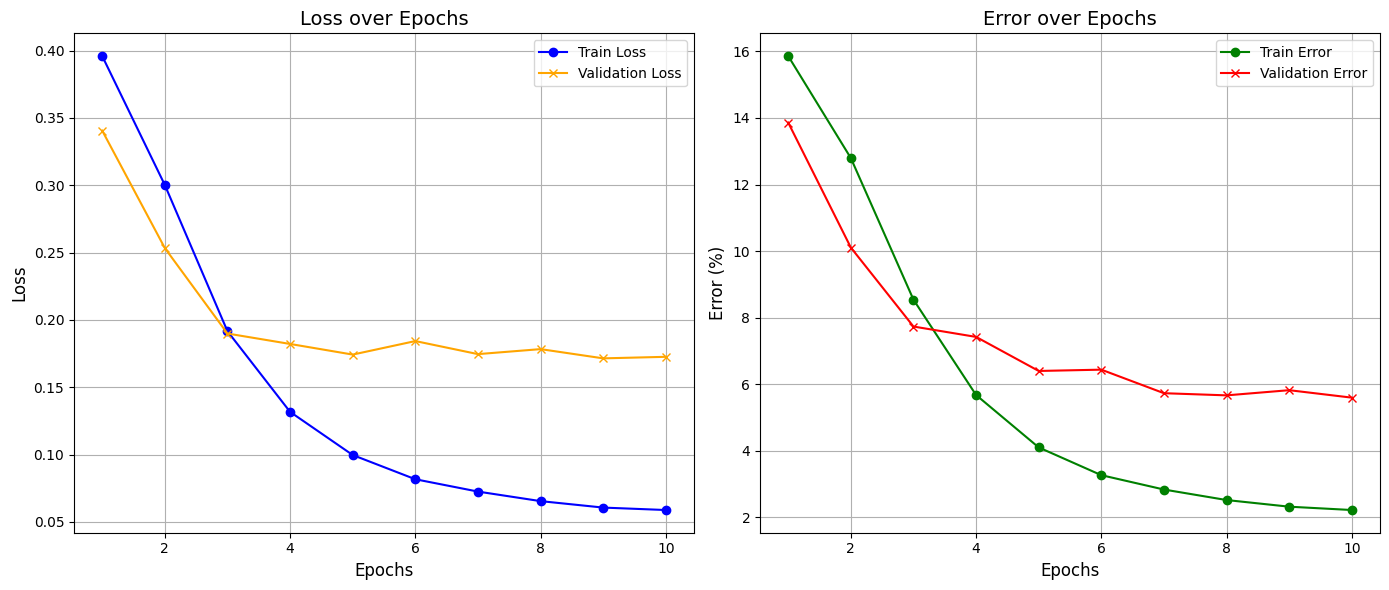
\includegraphics[width=\linewidth]{imgs/results_lr_0.00232.png}
        \caption{Training progress of the best model found}
        \label{fig:bestModel}
    \end{figure}\\
    The best model parameters, found during the random search, were determined to be a learning rate of 0.0232 and a dropout probability of 0.25\%. Initial observations, as shown in Figure \ref{fig:bestModel}, indicate that the error values recorded during the training process suggest commendable performance. The training curves show a consistent decrease in error rates, suggesting that the model has learned effectively.\\\\
    However, when the model was evaluated on the unbalanced test set, it showed an error rate, based on the accuracy, of around 13\%. This discrepancy in performance can be attributed to the different class distributions present in the training and test sets. While the training set was more balanced to ensure equal representation of all classes, the test set retained its natural distribution, which is skewed toward the drama class. This imbalance can significantly affect the model's performance, as it may have learned to predict certain classes more accurately than others based on their representation in the training data. Also, the shift in the number of genres per movie created during the balancing process could have an impact on the trained model. This suggests that other metrics for validating model performance should be considered, such as the micro and macro \textit{f1-score}, which combines precision and recall into a single metric. The macro \textit{f1-score} calculates the f1-score for each class independently and then takes the average, treating all classes equally. This is useful for understanding performance across all classes without being influenced by class frequency. On the other hand, the micro \textit{f1-score} aggregates the contributions of all classes to calculate the average \textit{f1-score}. This approach gives more weight to classes with more samples, which more accurately reflects overall performance when the data set that is unbalanced. The best found model has a very low training error (0.910\%) and high training \textit{f1 scores} (micro: 0.964, macro: 0.968), indicating a good fit to the training data. However, the test error is much higher (14.170\%) with low test \textit{f1-scores} (micro: 0.213, macro: 0.101), indicating overfitting. The low macro F1 score on the test set indicates difficulties with less frequent class.\\\\
    This poor performance on the test set highlights the importance of considering the class distribution. It suggests that while the model performs well on a balanced dataset, its ability to generalize to real-world, unbalanced scenarios is limited. Furthermore, this finding suggests the need to employ additional techniques, such as stratified sampling or class weighting, to ensure model robustness across different distributions, as well as a change in model architecture and consider a larger amount of data.
    \begin{figure}[h!]
        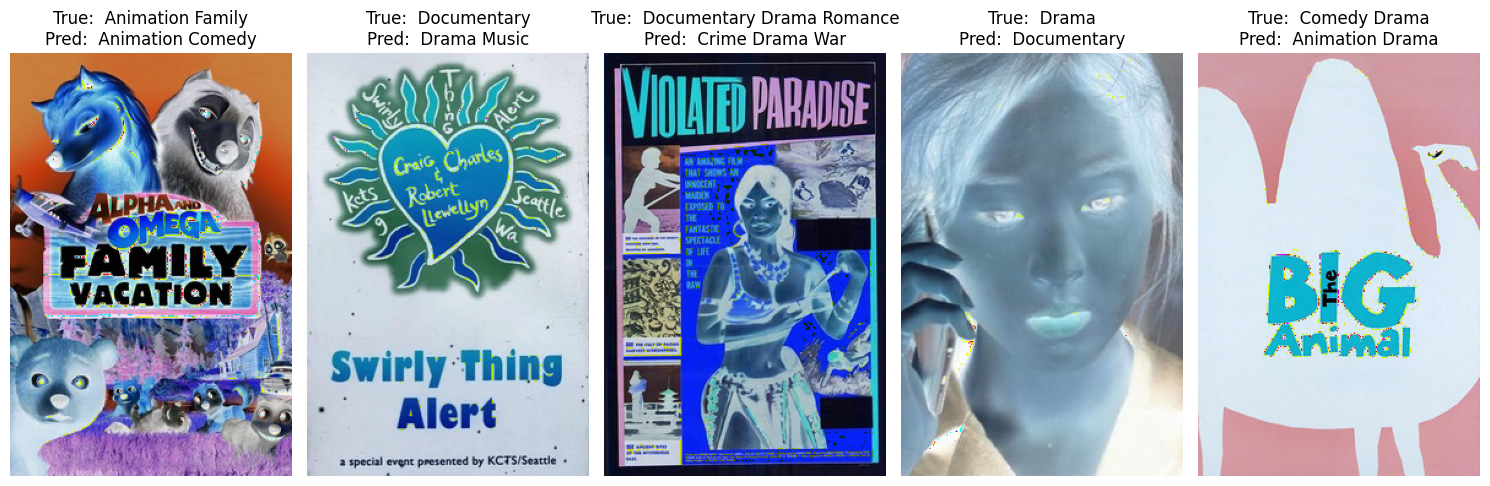
\includegraphics[width=\linewidth]{imgs/prediction_visualisation.png}
        \caption{Visualization of 5 examples from the test dataset and the corresponding predictions from the model}
        \label{fig:visualisationPrediction}
    \end{figure}\\
    A more visual and qualitative investigation reveals decent results (see fig. \ref{fig:visualisationPrediction}). Since the predicted genres for the examples in the test set can be considered to be in the same area as the true genres. 

\pagebreak
\bibliographystyle{abbrv}
\bibliography{references}  % need to put bibtex references in references.bib 
\end{document}